\pgfplotsset{compat=1.9}

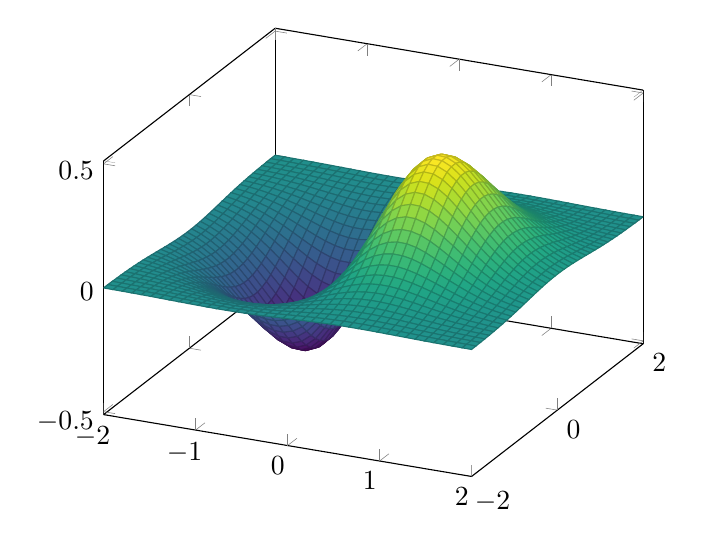
\begin{tikzpicture}
  \begin{axis}
    \addplot3[surf, colormap/viridis, domain=-2:2, samples=40] {x * exp(-x^2-y^2)};
  \end{axis}
\end{tikzpicture}

% Notes:
% When using "fill=white" instead of "colormap/viridis", all the factes are painted white such that 
% it looks like a cheaper variant of a surface plot. Using less than 40 samples makes it look rather
% rough. Uisng the "smooth" option doesn't work for this - apparently, this is only for curves and 
% not for surfaces.
